\section{Input linguistic variables}

\subsection{myEnergy}

The linguistic variable \emph{myEnergy} is the player's energy level and determines whether or not the player has \emph{lowEnergy} or \emph{highEnergy} remaining. The universe of disclosure for \emph{myEnergy} is between 0 joules and 10,000 joules, the amount of energy that all saucers begin with.

\begin{figure}[H]
\centering
\caption{\emph{myEnergy} fuzzy sets}
\includegraphics[scale=0.08]{./img/pdf/myEnergySets.pdf}
\end{figure}

\subsection{Target variables}

The sensor returns a list of all the enemy saucers currently in the battle space. This controller only considers the closest saucer as the target, and ignores all other saucers in the list.

\subsubsection{targetDist}

The linguistic variable \emph{targetDist} is the distance from the player to the target. The universe of disclosure for \emph{targetDist} is between 0m and 4802.3m, and the fuzzy sets are defined as \emph{close}, \emph{near}, and \emph{far}.

\begin{figure}[H]
\centering
\caption{\emph{targetDist} fuzzy sets}
\includegraphics[scale=0.08]{./img/pdf/targetDistSets.pdf}
\end{figure}

\subsubsection{targetAspect}

The linguistic variable \emph{targetAspect} is the direction of the target in relation to the player. The universe of disclosure for \emph{targetAspect} is between -360$^{\circ}$ and +360$^{\circ}$. Positive values rotate to the left, and negative values rotate to the right. The fuzzy sets selected relate to clock positions, similar to what fighter pilots might call out in combat. There are three twelve o'clock positions due to the two revolutions between -360$^{\circ}$ and +360$^{\circ}$.

\begin{figure}[H]
\centering
\caption{\emph{targetAspect} fuzzy sets}
\includegraphics[scale=0.08]{./img/pdf/targetAspectSets.pdf}
\end{figure}

\subsubsection{targetAngleOff}

The linguistic variable \emph{targetAngleOff} relates to the target's current heading, in relation to the player's current heading. For example, if the target is heading towards the player perpendicularly from the right, the target's angle-off would be +90$^{\circ}$. Similarly, if the target has the exact same heading as the player, the target's angle-off would be 0$^{\circ}$. Again, positive values rotate to the left, and negative values rotate to the right. The universe of disclosure is between -360$^{\circ}$ and +360$^{\circ}$. The fuzzy sets selected mimic clock positions, similar to \emph{targetAspect}, however are named with degree values. A merge is when the player and target have opposite angle-off's, ie. 180$^{\circ}$. In this situation, if the player and target were in front of each other, they would facing each other, and would be about to directly pass each other, in a ``merge''.

\begin{figure}[H]
\centering
\caption{\emph{targetAngleOff} fuzzy sets}
\includegraphics[scale=0.08]{./img/pdf/targetAngleOffSets.pdf}
\end{figure}

\subsubsection{targetEnergyDiff}

The linguistic variable \emph{targetEnergyDiff} relates to the difference between the player's energy and the current target's energy. The universe of disclosure for \emph{targetEnergyDiff} is between -10,000j and +10,000j. The fuzzy sets selected for this linguistic variable are \emph{losing} and \emph{winning}.

\begin{figure}[H]
\centering
\caption{\emph{targetEnergyDiff} fuzzy sets}
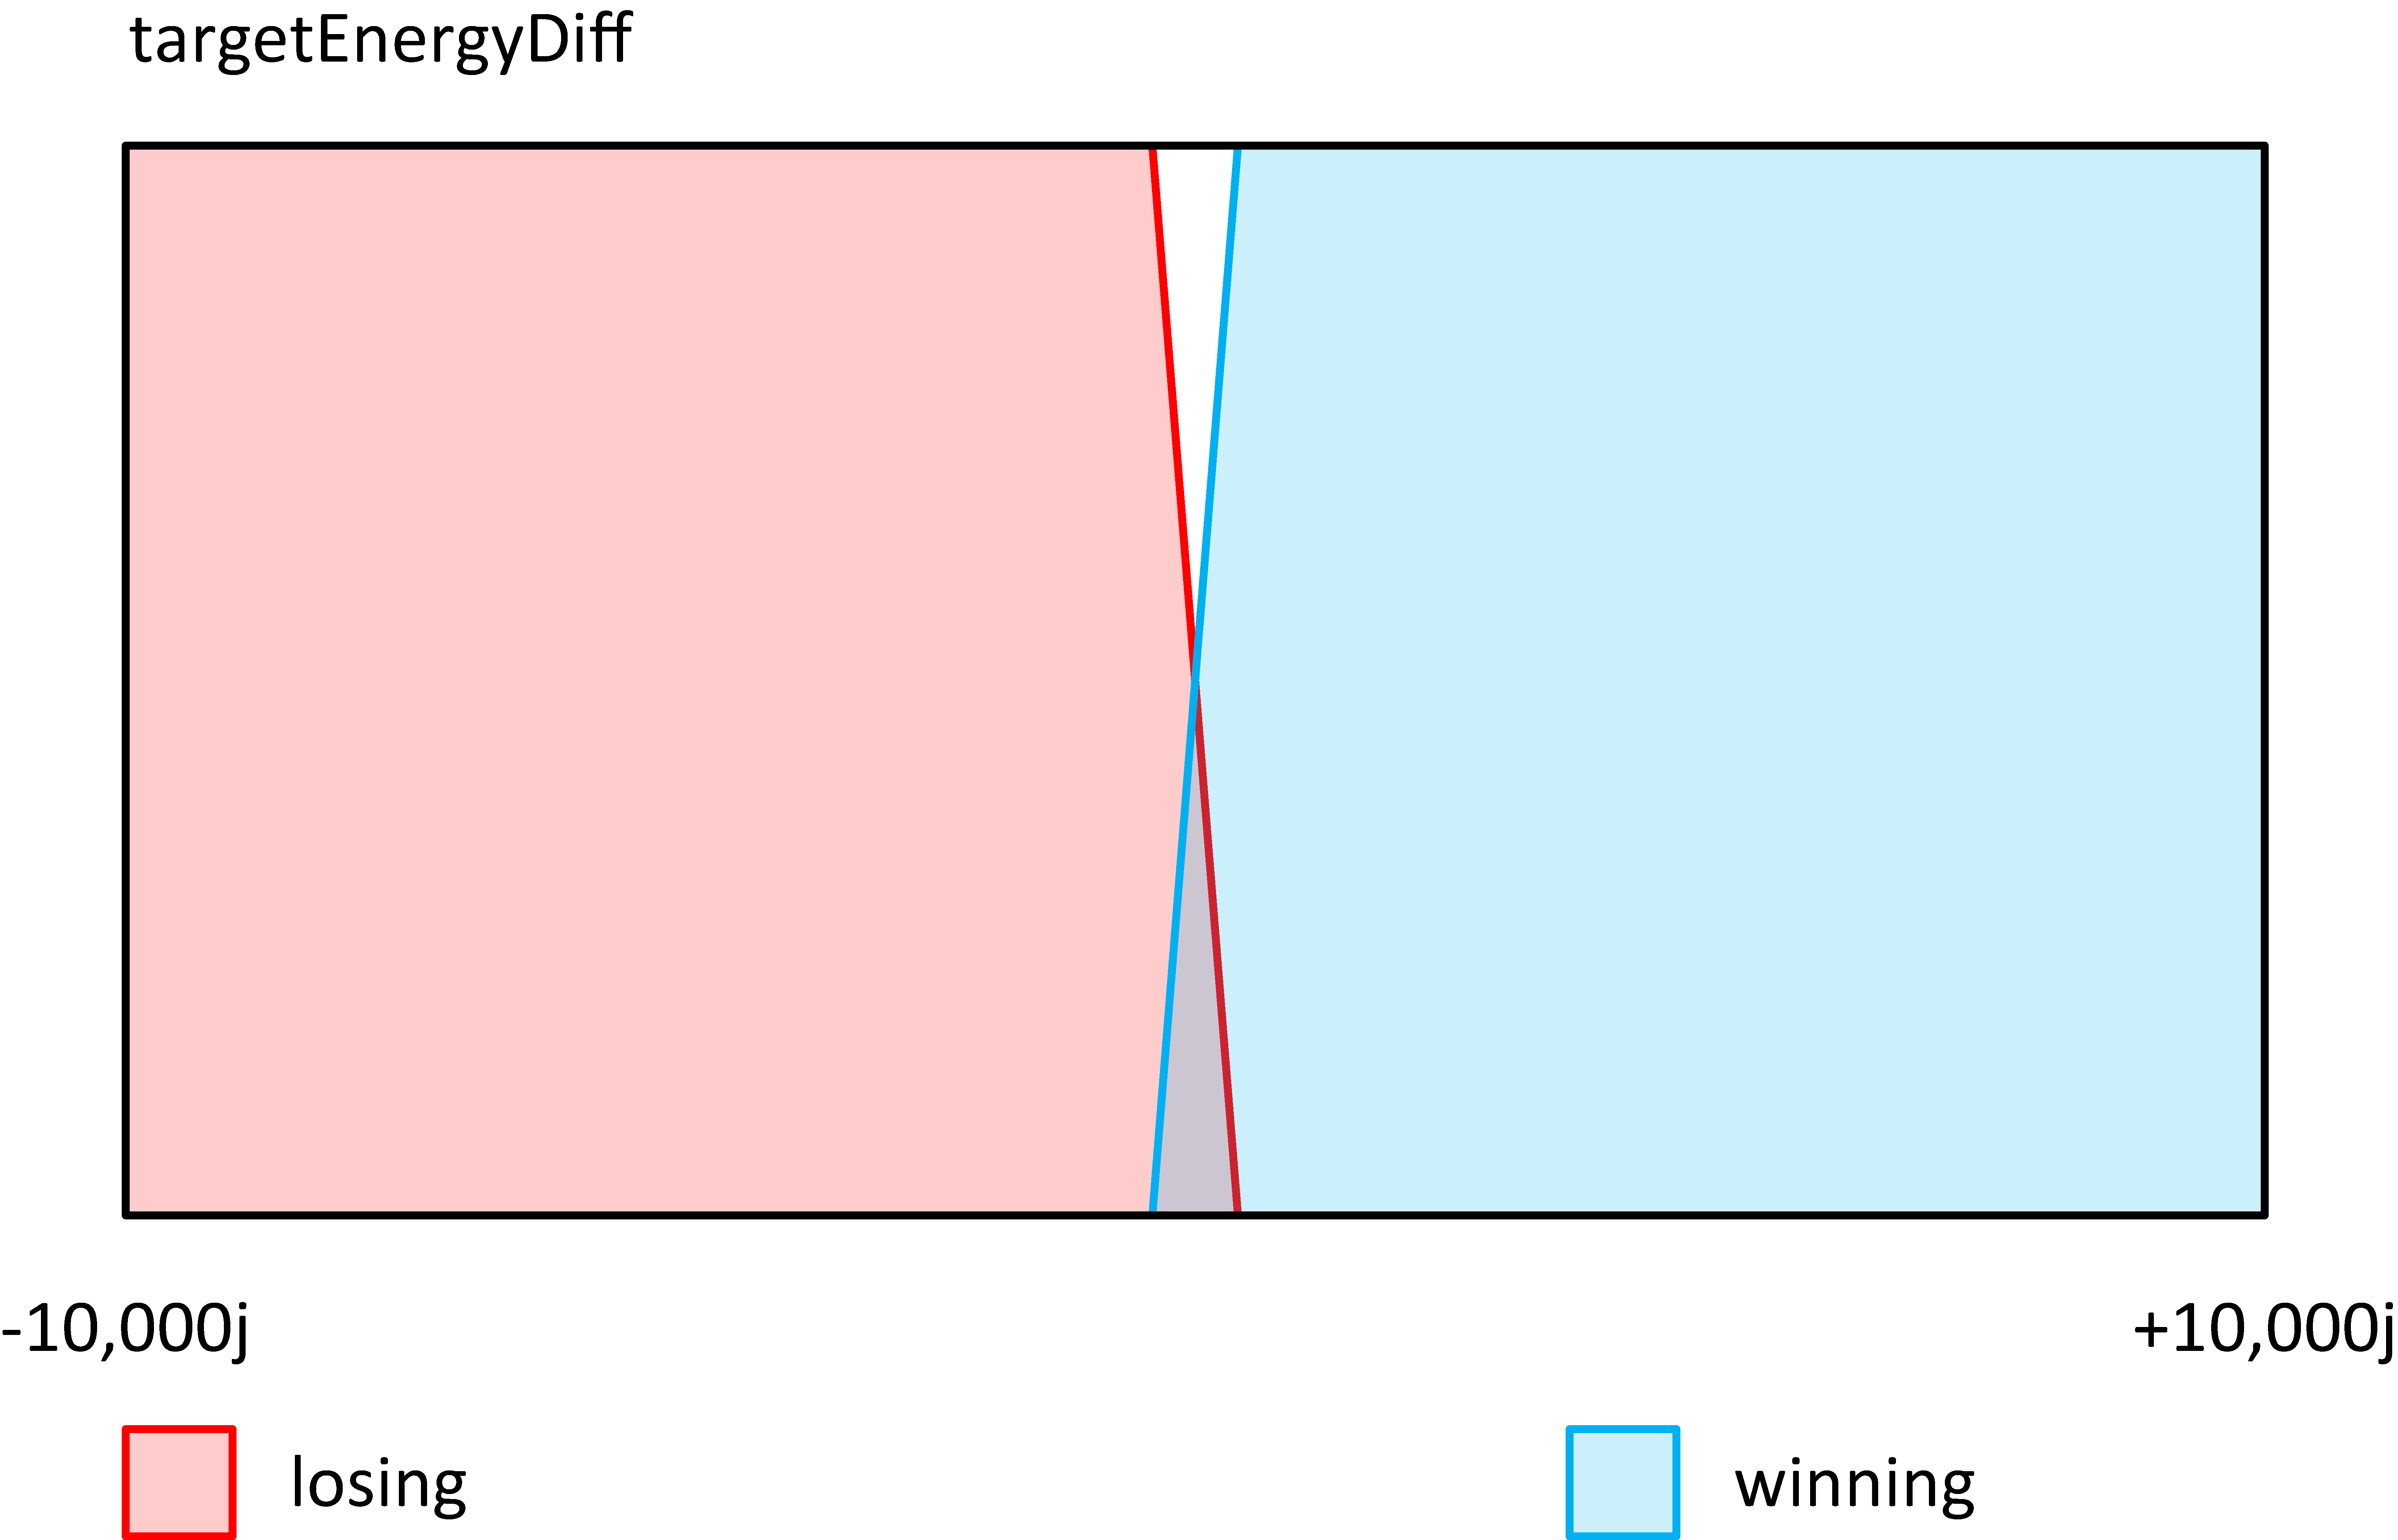
\includegraphics[scale=0.08]{./img/pdf/targetEnergyDiffSets.pdf}
\end{figure}

\subsection{Blast variables}

The sensor returns a list of all energy blasts currently in the battle space. This controller only considers the closest energy blast to dodge, and ignores all other blasts in the list.

\subsubsection{blastDist}

The linguistic variable \emph{blastDist} is the distance from the player to the energy blast. The universe of disclosure for \emph{blastDist} is between 0m and 4802.3m, and the fuzzy sets are defined as \emph{close} and \emph{far}.

\begin{figure}[H]
\centering
\caption{\emph{blastDist} fuzzy sets}
\includegraphics[scale=0.08]{./img/pdf/blastDistSets.pdf}
\end{figure}

\subsubsection{blastAspect}

The linguistic variable \emph{blastAspect} is similar to \emph{targetAspect}, but relates to the direction from the player to the energy blast. Similar fuzzy sets, based on the clock analogy have been used.

\begin{figure}[H]
\centering
\caption{\emph{blastAspect} fuzzy sets}
\includegraphics[scale=0.08]{./img/pdf/blastAspectSets.pdf}
\end{figure}

\subsubsection{blastAngleOff}

The linguistic variable \emph{blastAngleOff} is similar to \emph{targetAngleOff}, but references the current heading of the energy blast in relation to the player's heading. Similar fuzzy sets have also been used.

\begin{figure}[H]
\centering
\caption{\emph{blastAngleOff} fuzzy sets}
\includegraphics[scale=0.08]{./img/pdf/blastAngleOffSets.pdf}
\end{figure}

\subsection{Powerup variables}

The sensor returns a list of all powerups that currently exist in the battle space. To conserve energy, this controller only reacts to powerups only if they are nearby, and assumes that powerups that are far would most likely be consumed by an enemy by the time the player arrives.

\subsubsection{powerUpDist}

The linguistic variable \emph{powerUpDist} is the distance between the target and the powerup. Similar to \emph{targetDist}, the universe of disclosure is between 0m and 4802.3m. Similar fuzzy sets have also been used.

\begin{figure}[H]
\centering
\caption{\emph{powerUpDist} fuzzy sets}
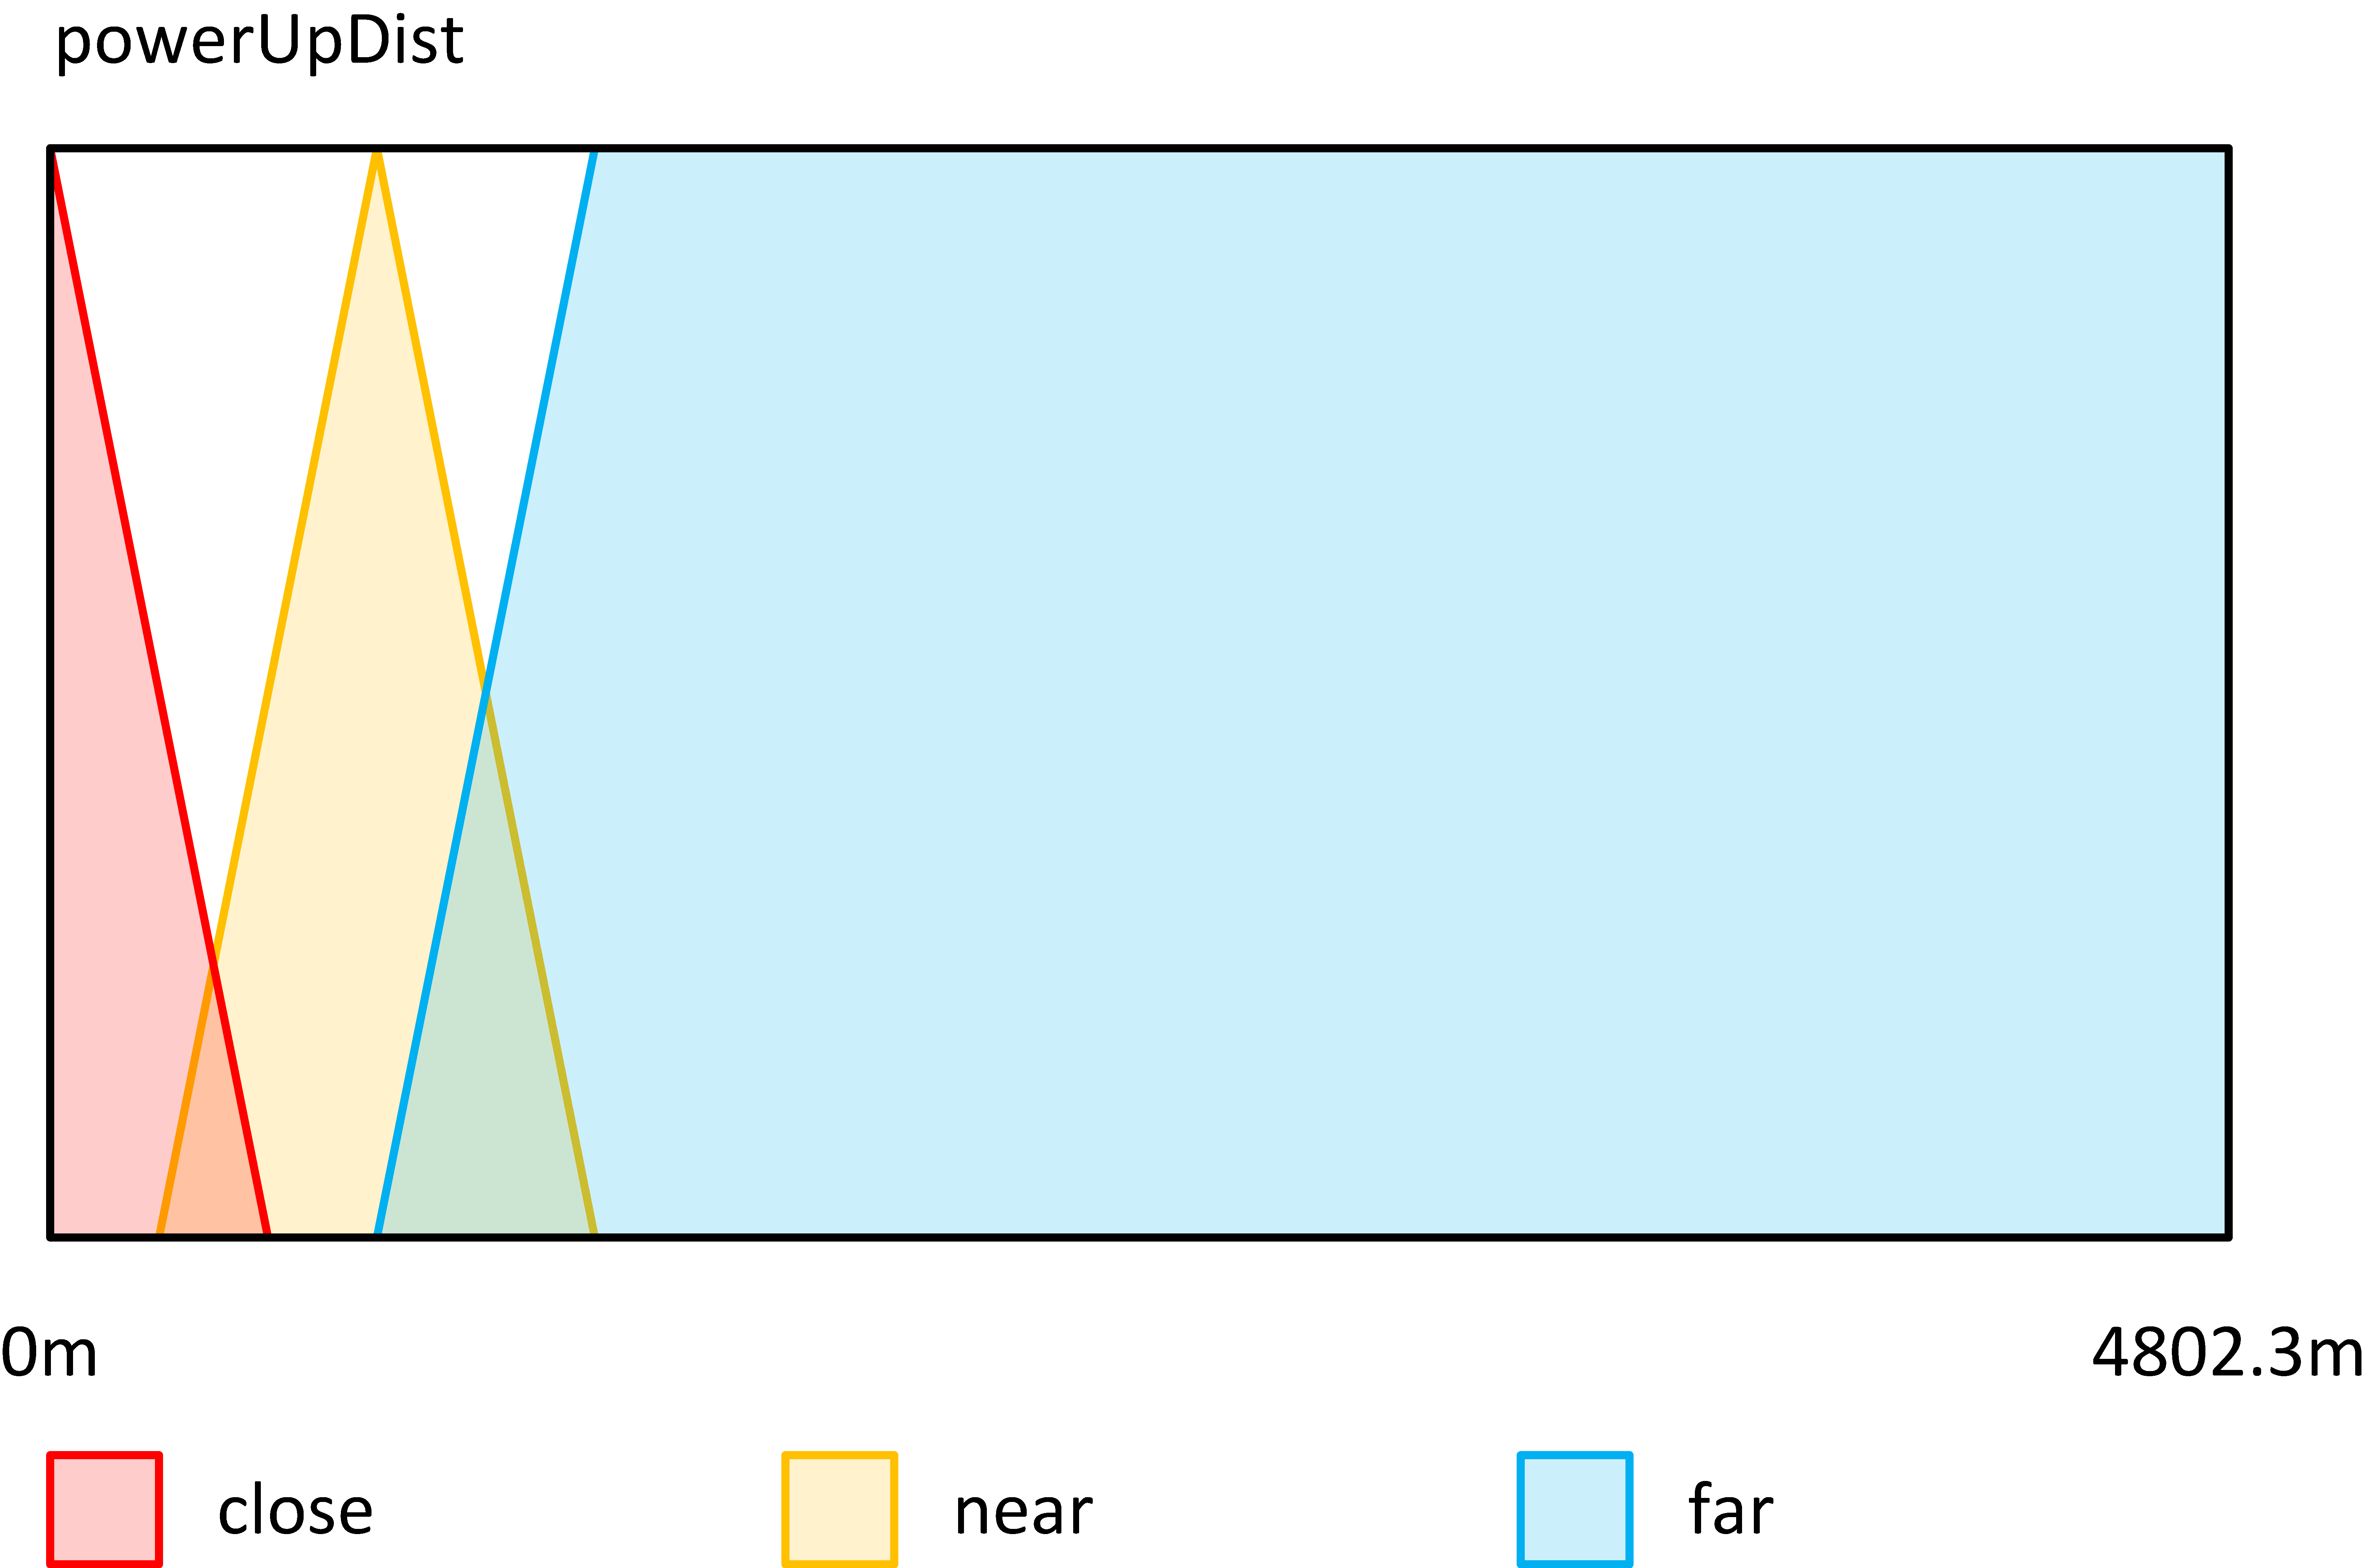
\includegraphics[scale=0.08]{./img/pdf/powerUpDistSets.pdf}
\end{figure}

\subsubsection{powerUpAspect}

The linguistic variable \emph{powerUpAspect} is the direction of the powerup in relation to the player. Again, the clock analogy has been used to determine the fuzzy sets. However, the angle-off of the powerup is not considered, since it is stationary and does not change its heading.

\begin{figure}[H]
\centering
\caption{\emph{powerUpAspect} fuzzy sets}
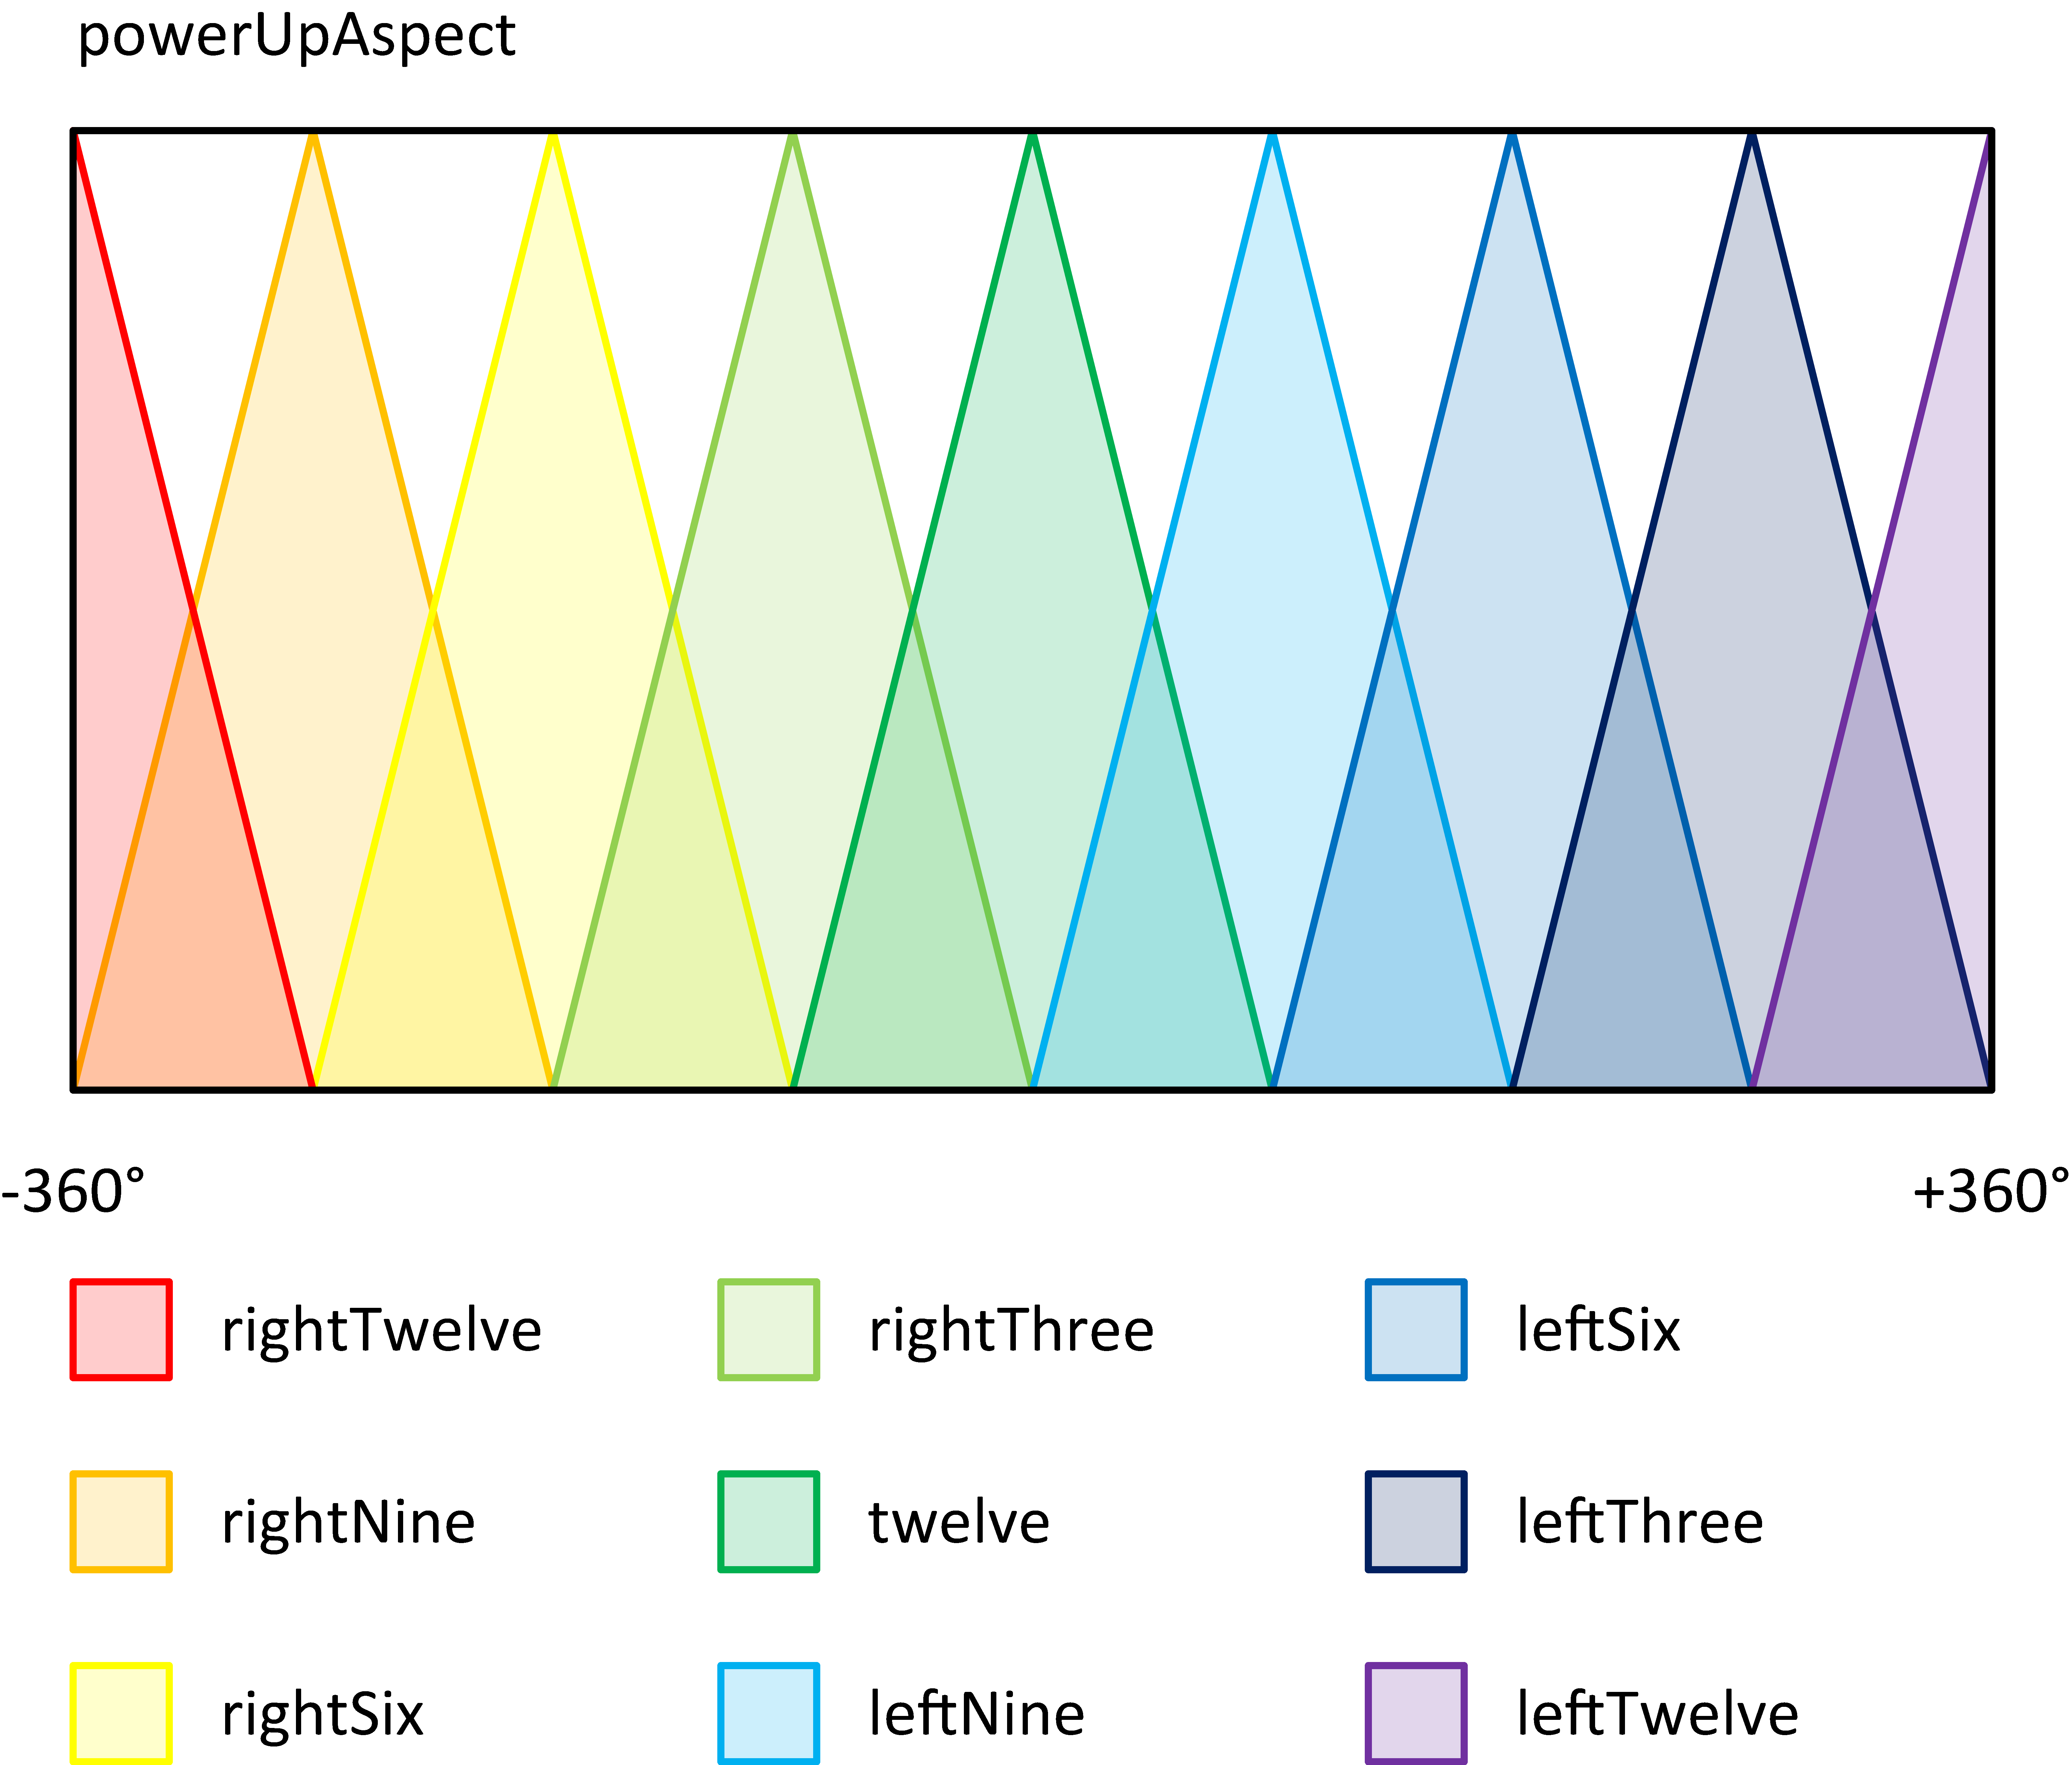
\includegraphics[scale=0.08]{./img/pdf/powerUpAspectSets.pdf}
\end{figure}

\section{Output linguistic variables}

Due to the fact that the fuzzy logic API does not provide a method to prioritize rules, defensive and offensive versions of some output linguistic variables have been defined. Boolean variables are defined, which are then tested to determine which version of the rule is fired, during a given situation.

For example, the defensive turn rule only considers the blast linguistic variables as input, whereas the offensive turn rule considers both target and blast linguistic variables.

\subsection{Defensive rules}

\subsubsection{defensiveTurn}

The \emph{defensiveTurn} linguistic variable defines which heading the saucer will take, in degrees, according to the rules that govern defensive turning. The linguistic variables used as input for \emph{defensiveTurn} are: \mintinline{console}{layerVar = blastDist}, \\ \mintinline{console}{rowVar = blastAngleOff}, and \mintinline{console}{colVar = blastAspect}, creating a 3D rule matrix. Note that \emph{r} and \emph{l} represent right and left in the table.
\\
\\
For example: IF (close) AND (rightSix) AND (zero) THEN (-90) \\
In other words, IF the energy blast is close, AND it is behind the player, AND it's heading towards the player, THEN turn right for 90$^{\circ}$.

\begin{table}[H]
\centering
\caption{\emph{defensiveTurn} \emph{close}}
\label{Turn rule table}
\begin{tabular}{r|r|r|r|r|r|r|r|r|r}
 		& rTwelve 	& rNine 	& rSix 		& rThree 		& twelve 	& lNine 	& lSix 		& lThree	& lTwelve		\\ \hline
rZero	& 0			& 0			& -90		& 0 		 	& 0			& 0			& +90	 	& 0			& 0				\\
r270	& +90		& 0			& 0			& +180			& +90		& 0			& 0			& +180		& +90			\\
rMerge	& 0			& 0			& -90	 	& 0				& 0			& 0			& +90		& 0			& 0				\\
r90		& +90		& -180		& 0 		& 0				& -90		& -180		& 0			& 0			& +90			\\
zero 	& 0			& 0 		& -90 		& 0				& 0			& 0			& +90		& 0			& 0				\\
l90 	& -90		& 0 		& 0			& +180			& +90		& 0			& 0			& +180		& -90			\\
lMerge	& 0			& 0 		& -90 		& 0				& 0			& 0			& +90		& 0			& 0				\\
l270 	& -90		& -180 		& 0			& 0				& -90		& -180		& 0			& 0			& -90			\\
lZero 	& 0			& 0 		& -90	 	& 0				& 0			& 0  		& +90		& 0			& 0				\\
\end{tabular}
\end{table}

\begin{table}[H]
\centering
\caption{\emph{defensiveTurn} \emph{far}}
\label{Turn rule table}
\begin{tabular}{r|r|r|r|r|r|r|r|r|r}
 		& rTwelve 	& rNine 	& rSix 		& rThree 	& twelve 	& lNine 	& lSix 		& lThree	& lTwelve	\\ \hline
rZero	& 0			& 0			& 0			& 0 	 	& 0			& 0			& 0	 		& 0			& 0			\\
r270	& 0			& 0			& 0			& 0			& 0			& 0			& 0			& 0			& 0			\\
rMerge	& 0			& 0			& 0	 		& 0			& 0			& 0			& 0			& 0			& 0			\\
r90		& 0			& 0			& 0 		& 0			& 0			& 0			& 0			& 0			& 0			\\
zero 	& 0			& 0 		& 0	 		& 0			& 0			& 0			& 0			& 0			& 0			\\
l90 	& 0			& 0 		& 0			& 0			& 0			& 0			& 0			& 0			& 0			\\
lMerge	& 0			& 0 		& 0	 		& 0			& 0			& 0			& 0			& 0			& 0			\\
l270 	& 0			& 0	 		& 0 		& 0			& 0			& 0			& 0			& 0			& 0			\\
lZero 	& 0			& 0 		& 0	 		& 0			& 0			& 0  		& 0			& 0			& 0			\\
\end{tabular}
\end{table}

The far rules have zero values so that the player does not react and maintains current heading when the energy blast is far, and is not a threat.

\subsubsection{defensiveSpeed}

The \emph{defensiveSpeed} linguistic variable defines how fast the saucer will travel, according to the rules that govern defensive speed. The linguistic variables used for input for \emph{defensiveSpeed} are: \mintinline{console}{layerVar = blastDist}, \mintinline{console}{rowVar = blastAngleOff}, and \mintinline{console}{colVar = blastAspect}, creating a 3D rule matrix.
\\
\\
For example: IF (close) AND (rightSix) AND (zero) THEN (125) \\
In other words, IF the energy blast is close, AND it is behind the player, AND it's heading towards the player, THEN speed is 125.

\begin{table}[H]
\centering
\caption{\emph{defensiveSpeed} \emph{close}}
\label{Turn rule table}
\begin{tabular}{r|r|r|r|r|r|r|r|r|r}
 		& rTwelve 	& rNine 	& rSix 		& rThree 		& twelve 	& lNine 	& lSix 		& lThree	& lTwelve		\\ \hline
rZero	& 50		& 125		& 125		& 125 		 	& 50		& 125		& 125 		& 125		& 50			\\
r270	& 50		& 125		& 50		& 125			& 50		& 125		& 50		& 125		& 50			\\
rMerge	& 50		& 125		& 50	 	& 125			& 125		& 125		& 50		& 125		& 50			\\
r90		& 50		& 125		& 50 		& 125			& 125		& 125		& 50		& 125		& 50			\\
zero 	& 50		& 125 		& 125 		& 125			& 50		& 125		& 125		& 125		& 50			\\
l90 	& 50		& 125 		& 50		& 125			& 125		& 125		& 50		& 125		& 50			\\
lMerge	& 50		& 125 		& 50	 	& 125			& 125		& 125		& 50		& 125		& 50			\\
l270 	& 50		& 125	 	& 50 		& 125			& 50		& 125		& 50		& 125		& 50			\\
lZero 	& 50		& 125 		& 125	 	& 125			& 50		& 125  		& 125		& 125		& 50			\\
\end{tabular}
\end{table}

\begin{table}[H]
\centering
\caption{\emph{defensiveSpeed} \emph{far}}
\label{Turn rule table}
\begin{tabular}{r|r|r|r|r|r|r|r|r|r}
 		& rTwelve 	& rNine 	& rSix 		& rThree 		& twelve 	& lNine 	& lSix 		& lThree	& lTwelve		\\ \hline
rZero	& 50		& 50		& 75		& 50 		 	& 50		& 50		& 75 		& 50		& 50			\\
r270	& 50		& 50		& 50		& 75			& 50		& 50		& 50		& 75		& 50			\\
rMerge	& 50		& 50		& 50	 	& 50			& 75		& 50		& 50		& 50		& 50			\\
r90		& 50		& 75		& 50 		& 50			& 75		& 75		& 50		& 50		& 50			\\
zero 	& 50		& 50 		& 75 		& 50			& 50		& 50		& 75		& 50		& 50			\\
l90 	& 50		& 50 		& 50		& 75			& 75		& 50		& 50		& 75		& 50			\\
lMerge	& 50		& 50 		& 50	 	& 50			& 75		& 50		& 50		& 50		& 50			\\
l270 	& 50		& 75	 	& 50 		& 50			& 50		& 75		& 50		& 50		& 50			\\
lZero 	& 50		& 50 		& 75	 	& 50			& 50		& 50  		& 75		& 50		& 50			\\
\end{tabular}
\end{table}

\subsection{Offensive rules}

\subsection{Neutral}

\subsubsection{getPowerTurn}

